The partial differential equation
\begin{equation}
(2-x^2)\frac{\partial^2 u}{\partial x^2}
+
2x^2y^2\frac{\partial^2 u}{\partial x\partial y}
+
(2-y^2)\frac{\partial^2 u}{\partial y^2}
=0
\label{70000008:pdgl}
\end{equation}
is to be solved in the domain
$\Omega=\{(x,y)\,|\, 0< x<1,\; 0<y<1\}$.
On the boundary of $\Omega$, the following values are given:
\begin{center}
\begin{tabular}{ccc}
\begin{minipage}{6cm}
\[
\begin{aligned}
&\text{für $0<x<1$:}&
u(x,0)&=\sin({\textstyle\frac\pi4} x)\\
&&
u(x,1)&=\sin({\textstyle\frac\pi4}(1-x))\\
\\
&\text{für $0<y<1$:}&
u(0,y)&=\sin({\textstyle\frac\pi4}y)\\
&&
u(1,y)&=\sin({\textstyle\frac\pi4}(1-y))
\end{aligned}
\]
\end{minipage}
&\qquad\qquad&
\begin{minipage}{8cm}
\begin{center}
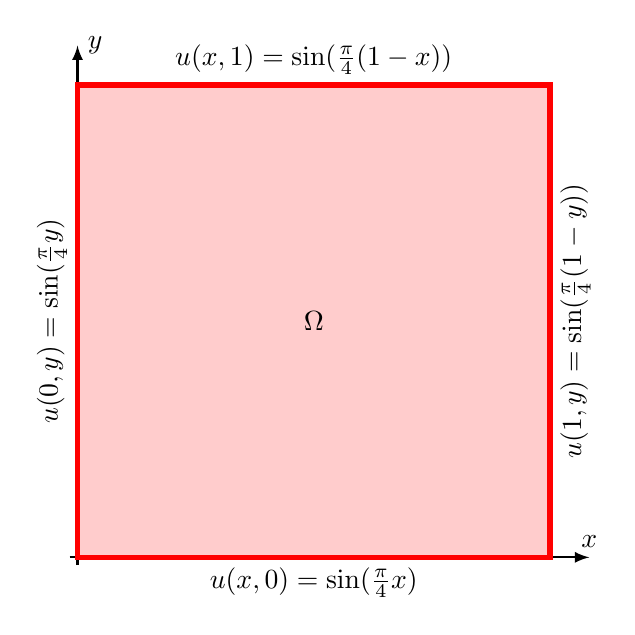
\begin{tikzpicture}[>=latex,thick]
\fill[color=red!20] (0,0) rectangle (6,6);
\draw[->] (-0.1,0) -- (6.5,0) coordinate[label={$x$}];
\draw[->] (0,-0.1) -- (0,6.5) coordinate[label={right:$y$}];
\draw[color=red,line width=2pt] (0,0) rectangle (6,6);
\node at (3,6) [above] {$u(x,1) = \sin(\frac{\pi}4(1-x))$};
\node at (3,0) [below] {$u(x,0) = \sin(\frac{\pi}4x)$};
\node at (0,3) [above,rotate=90] {$u(0,y) = \sin(\frac{\pi}4y)$};
\node at (6,3) [below,rotate=90] {$u(1,y) = \sin(\frac{\pi}4(1-y))$};
\node at (3,3) {$\Omega$};
\end{tikzpicture}
\end{center}
\end{minipage}
\end{tabular}
\end{center}

The numerically computed solution has produced a value
$u(\frac12,\frac12)=0.72$.
Is that value plausible?

\begin{hinweis}
Don't try to solve the partial differential equation.
\end{hinweis}

\begin{loesung}
Such a statement regarding the size of individual values is possible
for elliptic partial differential equations because their homogenous
solutions satisify the maximum principle.

So we first check whether we do have an elliptic partial differential
equation.
For that purpose, we need the symbol matrix, which happens to be
\[
A=\begin{pmatrix}
2-x^2 &x^2y^2\\
x^2y^2&2-y^2
\end{pmatrix}.
\]
The partial differential equation is elliptic if the eigenvalues
have the same sign, or equivalently if the determinant of the matrix
is positive:
\[
\det A=\underbrace{(2-x^2)}_{> 1}\underbrace{(2-y^2)}_{> 1}-\underbrace{x^4y^4}_{< 1}>0
\]
Please note that in the interior of the domain, and that's the only
thing that counts, the inequality holds and the determinant is
positive.
It follows that the partial differential equation
\eqref{70000008:pdgl} is elliptic.

The maximum principle tells us now that the function values of $u$
in the interior cannot be larger than the boundary values.
The boundary values are values of the the function
$f(t)=\sin(\frac\pi4t)$ for $0<t<1$.
As the function
$\sin(\frac\pi4t)$ is monotonically increasing, the maximum
is $\sin\frac\pi4=\frac{\sqrt{2}}2=0.7071067811865$.
The solution of $u$ thus cannot exceed 
$\frac{\sqrt{2}}2$ anywhere in $\Omega$.
Thus the value found numerically for the point
$(\frac12,\frac12)$ contradicts the maximum principle.
\end{loesung}

\begin{diskussion}
This problem is analogous to
\ref{70000005} in the problem collection.
\end{diskussion}

\begin{bewertung}
Symbol matrix ({\bf S}) 1 pt,
determinant and trace ({\bf D}) 1 pt,
sign of eigenvalues ({\bf V}) 1 pt,
classification as elliptic PDE ({\bf E}) 1 pt,
maximum principle ({\bf M}) 1 pt,
contradiction to the maximum principle ({\bf W}) 1 pt.
\end{bewertung}
